%arara: lualatex: { branch: developer, interaction: errorstopmode,
%arara: --> shell: yes, synctex: yes }
%arara: makeglossaries if found('aux', '@istfilename')
%arara: biber: { options: [ '--wraplines' ] }

\documentclass[%
% aspectratio=169,
spanish,
mexico]{beamer}
\mode<presentation>

\usepackage{babel}

\usetheme[progressbar=foot]{metropolis}
% \usecolortheme{seahorse}
% \usetheme{Warsaw}
% \usecolortheme{albatross}

\setbeamercolor{figure}{fg==black!2,bg=mDarkTeal}

\usepackage{fontspec}
    \setmainfont{TeX Gyre Pagella}
    \setsansfont{TeX Gyre Heros}

\renewcommand{\familydefault}{\sfdefault} % Sans serif

\usepackage{csquotes}
\MakeAutoQuote{“}{”}

\usepackage{microtype}
\setlength{\parskip}{1em}
\usepackage{tabularray}
    \UseTblrLibrary{booktabs}
    \UseTblrLibrary{siunitx}
    \DefTblrTemplate{contfoot-text}{normal}{\itshape Continúa en la siguiente página}
    \SetTblrTemplate{contfoot-text}{normal}
    \DefTblrTemplate{conthead-text}{normal}{\itshape (Continuación)}
    \SetTblrTemplate{conthead-text}{normal}

\usepackage{siunitx}
\sisetup{separate-uncertainty,per-mode=symbol,detect-all}
\DeclareSIUnit{\angstrom}{\textup{\AA}}

\usepackage{glossaries}
    \makeglossaries{}

\usepackage[%
style=numeric,
backend=biber,
url=false]{biblatex}

\addbibresource[location=remote]{http://127.0.0.1:23119/better-bibtex/export/library?/1/library.biblatex}

\DeclareCiteCommand{\footcite}[\mkbibfootnote]
  {\usebibmacro{prenote}}
  {\printnames[family-given]{labelname}%
   \newunit
   \printfield{shortjournal}%
   \newunit
   \printfield{doi}%
   \printlabeldateextra}
  {\addsemicolon\space}
  {\usebibmacro{postnote}}

% \makeatletter
% \def\@makefnmark{}
% \makeatother      

\setbeamerfont{footnote}{size=\tiny,shape=\itshape}

\setbeamertemplate{footnote}{%
  \parindent 1em\noindent%
  \raggedright
  \insertfootnotetext\par%
}	

\usepackage[skins]{tcolorbox}
\usepackage{paralist}
\usepackage{cleveref}
\usepackage{subcaption}
\usepackage[colorinlistoftodos]{todonotes}
\usepackage{lineno}
\usepackage{rotating}
\usepackage{newfloat}
\usepackage{float}
\DeclareFloatingEnvironment[
   fileext=los,
   listname={List of Schemes},
   name=Scheme,
   placement=tbp,
   within=none % don't reset numbering
]{scheme}
\DeclareCaptionSubType{scheme}
\setcounter{secnumdepth}{5}

\begin{filecontents}[force]{abreviaturas.tex}
    \newacronym{DFT}{DFT}{Teoría del funcional de la densidad \textit{(del inglés ``Density Functional Theory'')}}
    \newacronym{TDDFT}{TDDFT}{Teoría del funcional de la densidad tiempo-dependiente \textit{(del inglés ``Time-Dependant Density Functional Theory'')}}
    \newacronym{FMR}{FMR}{Rotores Moleculares Fluorescentes \textit{(Del inglés ``Flurescent Molecular Rotor'')}}
    \newacronym{BOSCHIBA}{BOSCHIBA}{Bases de Schiff de Boro \textit{(del inglés ``\textsc{Bo}ron \textsc{Schi}ff \textsc{Ba}ses'')}}
    \newacronym{BODIPY}{BODIPY}{\textsc{bo}ron-\textsc{di}\textsc{py}rromethene}
    \newacronym{TICT}{TICT}{transferencia de carga intramolecular retorcida \textit{(del inglés ``twsited intramolecular charge transfer'')}}
    \newacronym{LE}{LE}{Local Excitado \textit{(del inglés ``locally exited'')}}
    \newacronym{MW}{MW}{Microondas \textit{(del inglés ``Microwave'')}}
    \newacronym{PES}{PES}{Superficie de Energía Potencial \textit{(del inglés ``Potential Energy Surface'')}}
    \newacronym{NBO}{NBO}{Orbitales Naturales de Enlace \textit{(del inglés ``Natural Bond Orbitals'')}}
    \newacronym{ICT}{ICT}{Transferencia de Carga Intramolecular \textit{(del inglés ``Intramolecular Charge Transfer'')}}
    \newacronym{VEE}{VEE}{Energía de Emisión Vertical \textit{(del inglés ``Vertical Emission Energy'')}}
    \newacronym{FMO}{FMO}{Orbitales Moleculares de Frontera \textit{(del inglés ``Frontier Molecular Orbitals'')}}
    \newacronym{HOMO}{HOMO}{Orbital Molecular de mas alta energía \textit{(del inglés ``Highest Occupied Molecular Orbital'')}}
    \newacronym{LUMO}{LUMO}{Orbital Molecular no ocupado de más baja energía \textit{(del inglés ``Lowest Unoccupied Molecular Orbital'')}}
    \newacronym{NMR}{NMR}{Resonancia Magnética Nuclear \textit{(del inglés ``Nuclear Magnetic Resonance'')}}
    \newacronym{CREST}{CREST}{\textit{Conformer-Rotamer Ensemble Sampling Tool}}
\end{filecontents}

\begin{filecontents}[force]{comandos.tex}
    % \newcommand{\invitro}{\textit{in-vitro}}
    \newcommand\scan{\(\text{r}^{2}\text{SCAN-3c}\)}
    
\end{filecontents}

\begin{filecontents}[force]{quimica.tex}
    \usepackage{chemmacros}
    \DeclareChemReactant{BO-gly}{name={BO-Gly}} % 1
    \DeclareChemReactant{BO-trp}{name={BO-Trp}} % 2
    \DeclareChemReactant{BO-tyr}{name={Bo-Tyr}} % 3
    \DeclareChemReactant{BO-phe}{name={BO-Phe}} % 4
    \DeclareChemReactant{trp}{name={\iupac{\laevus-triptófano}}, short={trp}}
    \DeclareChemReactant{phe}{name={\iupac{\laevus-fenilalanina}}, short={phe}}
    \DeclareChemReactant{tyr}{name={\iupac{\laevus-tirosina}}, short={tyr}}
    \DeclareChemReactant{gly}{name={glicina}, short={gly}}
    \DeclareChemReactant{aphb}{name={ácido fenil borinico}, short={\ch{PhB(OH)2}}}
    \DeclareChemReactant{2h1n}{name={\iupac{2-Hidroxi-1-naftaldehido}}, short={\iupac{2-Hidroxi-1-naftaldehido}}}
    \NewChemLatin\invitro{in vitro}
    \NewChemLatin\invivo{in vivo}
    \NewChemLatin\insilico{in silico}
    \DeclareChemTranslation{scheme-name}{spanish}{Esquema}
    \DeclareChemTranslation{scheme-list}{spanish}{Lista de esquemas}
    \DeclareChemTranslation{scheme}{spanish}{esquema}
    \DeclareChemTranslation{schemes}{spanish}{esquemas}
    \DeclareChemTranslation{Scheme}{spanish}{Esquema}
    \DeclareChemTranslation{Schemes}{spanish}{Esquemas}
    \chemsetup{language=spanish}
    % \renewcommand{\schemename}{Esquema}
    % \AtBeginDocument{
    % \renewcommand{\tablename}{Tabla}
    % }
    
    \AtBeginDocument{%
    \addto\captionsspanish{\renewcommand\listschemename{Índice de esquemas}}%
    \addto\captionsspanish{\renewcommand\schemename{Esquema}}%
    \csname captions\languagename\endcsname
}
    % \chemsetup[reactants]{printreactants-style=xltabular}
\end{filecontents}

%% LaTeX2e file `abreviaturas.tex'
%% generated by the `filecontents' environment
%% from source `PEAG-Protocolo_maestria' on 2023/09/17.
%%
    \newacronym{DFT}{DFT}{Teoría del funcional de la densidad \textit{(del inglés "Density Functional Theory")}}
    \newacronym{TDDFT}{TDDFT}{Teoría del funcional de la densidad tiempo-dependiente \textit{(del inglés "Time-Dependant Density Functional Theory")}}
    \newacronym{FMR}{FMR}{Rotores Moleculares Fluorescentes \textit{(Del inglés Flurescent Molecular Rotor)}}
    \newacronym{BOSCHIBA}{BOSCHIBA}{Bases de Schiff de Boro \textit{(del inglés "\textsc{Bo}ron \textsc{Schi}ff \textsc{Ba}ses")}}
    \newacronym{BODIPY}{BODIPY}{\textsc{bo}ron-\textsc{di}\textsc{py}rromethene}
    \newacronym{TICT}{TICT}{transferencia de carga intramolecular retorcida \textit{(del inglés "twsited intramolecular charge transfer")}}
    \newacronym{LE}{LE}{local excitado \textit{(del inglés "locally exited")}}

%% LaTeX2e file `comandos.tex'
%% generated by the `filecontents' environment
%% from source `Presentación-Protocolo-Maestria-PEAG' on 2023/11/14.
%%
    % \newcommand{\invitro}{\textit{in-vitro}}
    \newcommand\scan{\(\text{r}^{2}\text{SCAN-3c}\)}


%% LaTeX2e file `quimica.tex'
%% generated by the `filecontents' environment
%% from source `PEAG-Protocolo_maestria' on 2023/09/17.
%%
    \DeclareChemReactant{BO1}{name={BO1}, short={THF}}
    \DeclareChemReactant{BO-trp}{name={triptófano}, short={BO-trp}}
    \DeclareChemReactant{BO-phe}{name={fenilalanina}, short={BO-phe}}
    \DeclareChemReactant{BO-tyr}{name={tirosina}, short={BO-tyr}}
    \DeclareChemReactant{BO-gly}{name={glicina}, short={BO-gly}}
    \NewChemLatin\invitro{in vitro}
    \NewChemLatin\insilico{in silico}
    \DeclareChemTranslation{scheme-name}{spanish}{Esquema}
    \DeclareChemTranslation{scheme-list}{spanish}{Lista de esquemas}
    \DeclareChemTranslation{scheme}{spanish}{esquema}
    \DeclareChemTranslation{schemes}{spanish}{esquemas}
    \DeclareChemTranslation{Scheme}{spanish}{Esquema}
    \DeclareChemTranslation{Schemes}{spanish}{Esquemas}
    \renewcommand{\schemename}{Esquema}


% \renewcommand{\iffootnote}{\scriptsize}

\title{Síntesis sustentable, caracterización química-fotofísica, y por DFT de BOSCHIBA derivadas de aminoácidos y su aplicación \invitro{}}
\subtitle{Protocolo de tesis de maestría}
\date{2023--11--30}
\author{Pablo E. Alanis}
\institute{Universidad Autónoma de Nuevo León, División de Posgrado}

\begin{document}
\maketitle

\begin{frame}[allowframebreaks]{Contenido}
	\tableofcontents
\end{frame}

% \begin{frame}
%     \begin{itemize}[<+- | alert@+>]
%         \item Se evaluó con \fbox{FabH} y \fbox{FabI}
%         \item Se determinó la afinidiad en los sitios activos de estas proteínas
%         \item Se usó SYBYL-X 2.0 para determinar la afinidad $K_b$
%     \end{itemize}
% \end{frame}

\section{Resumen}

\begin{frame}[standout]
	\small
	\vspace*{\fill}
	Se sintetizarán una serie de \gls{BOSCHIBA} derivadas de \reactant*{gly}, \reactant*{trp}, \reactant*{tyr} y \reactant*{phe}. Se caracterizarán por métodos espectroscópicos y se realizarán cálculos \insilico{} por medio de \gls{DFT} y \gls{TDDFT} para estudiar las propiedades fotofísicas de los compuestos y comprobar los mecanismos involucrados en el efecto supresor de la luminiscencia en dichos compuestos así como estudios de topológicos sobre los mismos. A su vez, se realizarán estudios de citotoxicidad y tinción \invitro{} para determinar su actividad biológica de los compuestos.
	\vspace*{\fill}
\end{frame}

\section{Introducción}
\begin{frame}{Introducción}
	\begin{itemize}[<+- | alert@+>]
		\item Interés en compuestos fluorescentes de boro;
		\item Amplio campo de aplicaciones;
		\item BODIPY comercialmente disponibles;
		      \begin{itemize}
			      \item Utilizados como agentes para la tinción celular:
			            \begin{enumerate}
				            \item ER-Tracker™ Green, y;
				            \item ER-Tracker™ Red.
			            \end{enumerate}
		      \end{itemize}
	\end{itemize}
\end{frame}

{
\setbeamercolor{background canvas}{fg=black!2, bg=white}
\begin{frame}{ER-Tracker™}
	\begin{scheme}[H]
		\centering
		\begin{subscheme}{0.45\linewidth}
			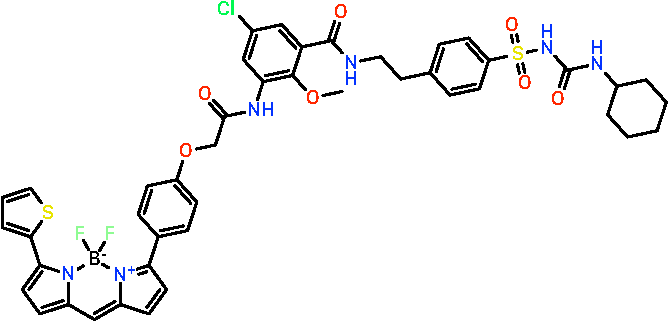
\includegraphics[width=\linewidth]{./Figuras/ER-Tracker_Blue.pdf}
			\caption{ER-Tracker™ Blue}
			\label{ER-Tracker_Blue}
		\end{subscheme}
		\hfill
		\begin{subscheme}{0.45\linewidth}
			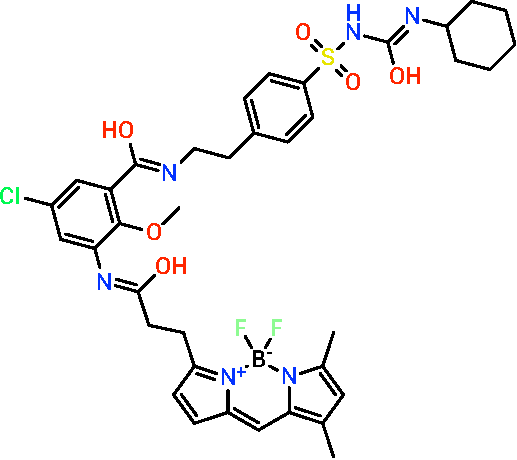
\includegraphics[width=\linewidth]{./Figuras/ER-Tracker_Green.pdf}
			\caption{ER-Tracker™ Green}
			\label{ER-Tracker_Green}
		\end{subscheme}
		\caption[ER-Trackers™]{\textit{Los ER-Tracker™ Green} y \textit{ER-Tracker™ Red} de Thermo Fischer Scientific™ son \gls{BODIPY} comerciales utilizados como agentes para la tinción celular.}
		\label{ER-Trackers}
	\end{scheme}
\end{frame}
}


\begin{frame}{Fluoróforos sensibles a la viscosidad i}
	\begin{itemize}[<+- | alert@+>]
		\item Los \gls{FMR} son fluoróforos sensibles a la viscosidad.
		\item Presentan una rotación libre que se vuelven fluorescentes.
		\item Aumentan la fluorescencia solo si su rotación se ve restringida.
	\end{itemize}
\end{frame}

\begin{frame}{Fluoróforos sensibles a la viscosidad ii}
	\begin{itemize}[<+- | alert@+>]
		\item Algunas interacciones de carácter intramolecular para detener la rotación de los \gls{FMR} son:
		      \begin{enumerate}[i.]
			      \item Formar interacciones de hidrógeno;\footcite{wuMultistageRotationalSpeed2018}
			      \item A través del impedimento estérico;\footcite{faulknerAllostericRegulationRotational2016} o
			      \item Por la formación de complejos estables con iones metálicos.\footcite{yadavViscochromicMechanochromicUnsymmetrical2019}
		      \end{enumerate}
	\end{itemize}
\end{frame}

\begin{frame}{Fluoróforos sensibles a la viscosidad iii}
	\begin{itemize}[<+- | alert@+>]
		\item Se ha determinado que la polaridad del solvente y la viscosidad del mismo afectan considerablemente la fluorescencia de los \gls{FMR}.
		\item El efecto que tiene la polaridad del solvente, aunque se sabe que es importante, no se ha logrado elucidar de forma aislada a la viscosidad.\footcite{haidekkerEffectsSolventPolarity2005}
	\end{itemize}
\end{frame}

\begin{frame}{Diseño de FMR}
    \begin{itemize}[<+- | alert@+>]
        \item Diferentes estrategias para el diseño de \gls{FMR} se han propuesto para realizar sensores de viscosidad altamente sensibles.
        \item Ejemplos incluyen: incorporando grupos rotacionales asimétricos,\footcite{leePyrrolicMolecularRotors2016} usando grupos con alta capacidad para rotar,\footcite{karpenkoPushPullDioxaborine2016} variación de puentes π-conjugados tipo \emph{push-pull},\footcite{karpenkoPushPullDioxaborine2016} la aplicación de rotadores di- o trímeros,\footcite{kimballBODIPYBODIPYDyad2015} y la introducción de dos rotadores distintos con diferentes capacidades rotacionales y electrondonantes.\footcite{rautTriazinebasedBODIPYTrimer2016}
    \end{itemize}
\end{frame}

\begin{frame}{Rendimiento y Contraste de FMR}
    \begin{itemize}[<+- | alert@+>]
        \item Obtener tanto una alta eficiencia de fluorescencia como un contraste fluorescente simultáneamente es muy difícil.
        \item El rendimiento cuántico y el contraste de fluorescencia de los \gls{FMR} están inversamente correlacionados, una relación llamada ``intensidad de fluorescencia---contraste".\footcite{leeFrontCoverFluorescent2018}
    \end{itemize}
\end{frame}

\begin{frame}{Variedad de FMR}
    \begin{itemize}
        \item En la actualidad existe una amplia variedad de \gls{FMR} derivados de compuestos de boro, donde los \gls{BODIPY} y los dioxaborinos son los protagonistas debido a su elevado rendimiento cuántico.
        \item Sin embargo, muestran algunas desventajas como la síntesis en varias etapas, condiciones de atmósfera anhidra y, en muchas ocasiones, una capacidad de contraste baja.\footcite{karpenkoPushPullDioxaborine2016,guptaBodipyBasedFluorescent2016,liBODIPYBasedTwoPhotonFluorescent2018,kimBorondifluorideComplexesHemicurcuminoids2016}
    \end{itemize}
\end{frame}

\begin{frame}{BOSCHIBA como FMR}
    \begin{itemize}[<+- | alert@+>]
        \item Recientemente, nuestro grupo de trabajo ha informado sobre la síntesis de \gls{BOSCHIBA} y su uso como \gls{FMR} en la detección de viscosidad y la bioimagen de células.\footcite{ibarra-rodriguezFluorescentMolecularRotors2017}
        \item Los resultados encontrados indican que los \gls{BOSCHIBA} pueden aumentar hasta 34 veces su valor de rendimiento cuántico en medios de alta viscosidad.
    \end{itemize}
\end{frame}

\begin{frame}{Mejoramiento del Contraste y la Bioimagen}
    \begin{itemize}[<+- | alert@+>]
        \item Para lograr mejorar el contraste de fluorescencia y la bioimagen celular, se diseñó una serie de \gls{BOSCHIBA} derivados de aminoácidos.
        \item Las moléculas presentan rotación libre a través del anillo fenilborónico, y el aminoácido podría dar una mayor compatibilidad y solubilidad en medios celulares.
    \end{itemize}
\end{frame}

\begin{frame}{Síntesis de Compuestos de Boro Fluorescentes}
    \begin{itemize}[<+- | alert@+>]
        \item Los compuestos de boro fluorescentes \textbf{1-4} se sintetizarán por una reacción multicomponente en \gls{MW}.
        \item El objetivo es tener altos rendimientos químicos en un tiempo de reacción corto.
        \item Este método resulta más eficiente y rápido en comparación con \gls{BOSCHIBA} similares reportados en la literatura sintetizados por métodos convencionales.
    \end{itemize}
\end{frame}

\begin{frame}{Compuestos a Sintetizar}
    \begin{figure}
        \centering
        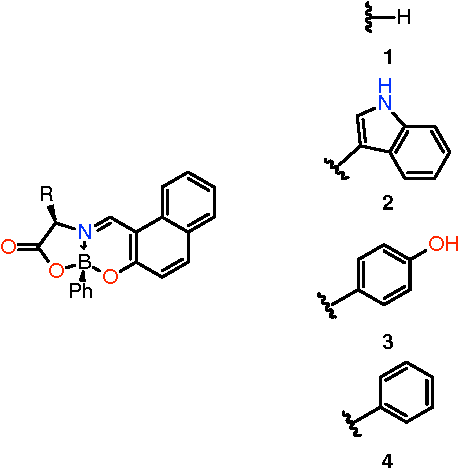
\includegraphics[width=0.5\linewidth]{./Figuras/Marcha.pdf}
        \caption{Compuestos que se sintetizarán en esta investigación.}
        \label{sch:marcha}
    \end{figure}
\end{frame}

\section{Antecedentes}
\begin{frame}[allowframebreaks]{Antecedentes}
\begin{figure}
    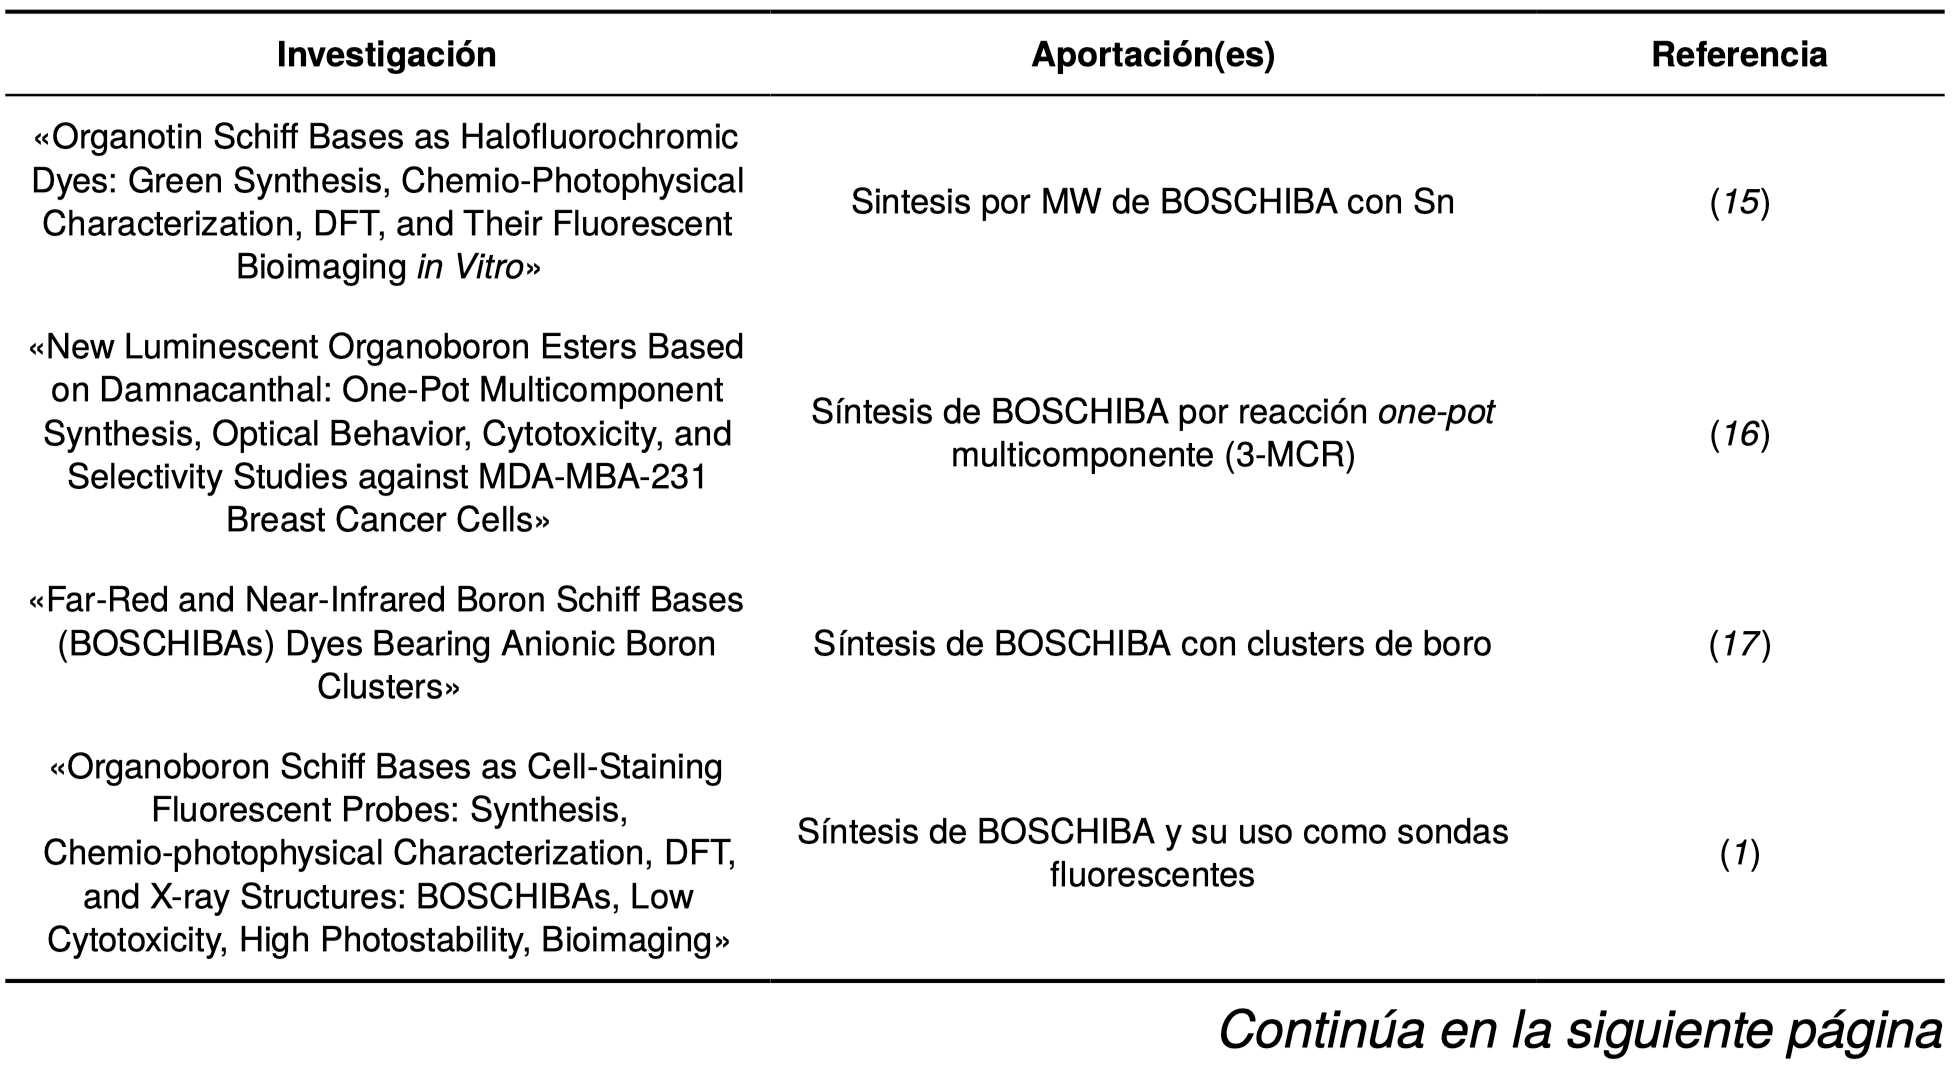
\includegraphics[width=0.95\linewidth]{./Figuras/t1.png}
\end{figure}
\framebreak
\begin{figure}
    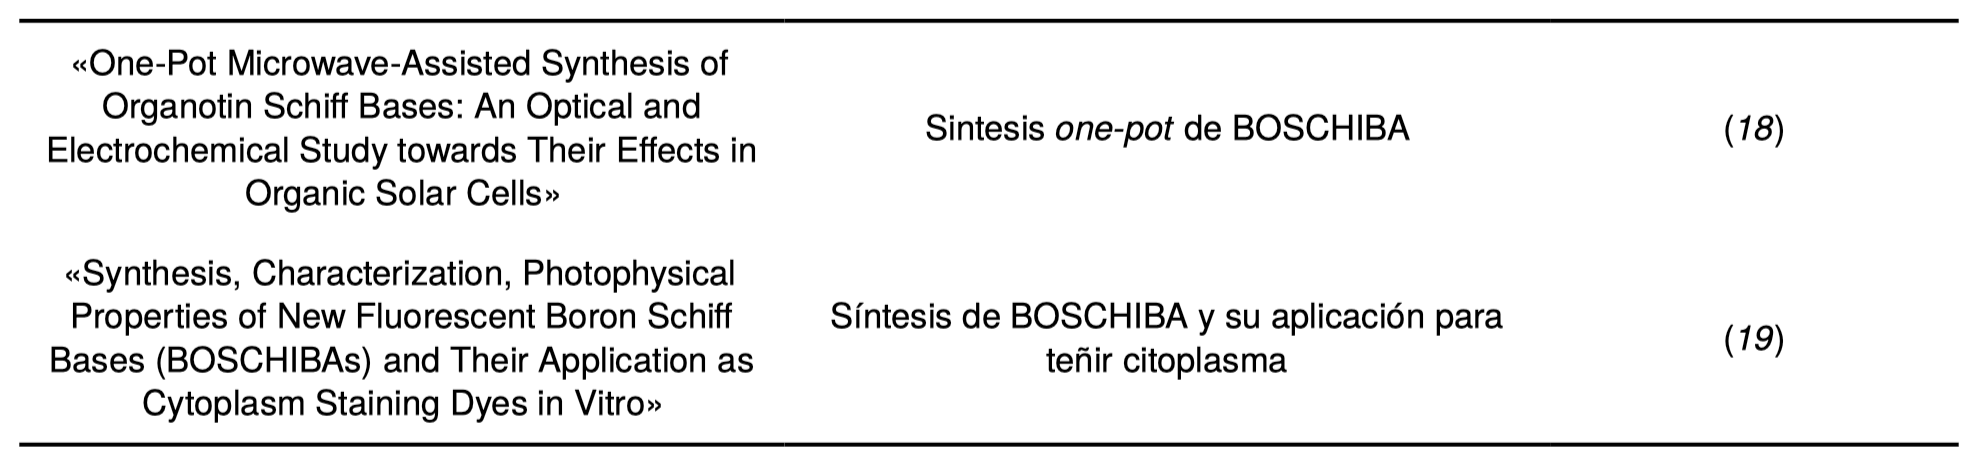
\includegraphics[width=0.95\linewidth]{./Figuras/t2.png}
\end{figure}
\end{frame}

\subsection{Análisis crítico de los antecedentes}

\begin{frame}{Investigación de Corona-López et al. (2017)}
    \begin{itemize}[<+- | alert@+>]
        \item Preparación de \gls{BOSCHIBA} por reacción de condensación.
        \item Incorporación de sustituyentes voluminosos para mejorar la estabilidad.
    \end{itemize}
\end{frame}

\begin{frame}{Investigación de Ibarra-Rodríguez et al. (2019)}
    \begin{itemize}[<+- | alert@+>]
        \item Uso de \gls{BOSCHIBA} para detección de células cancerígenas.
        \item Propuesta de síntesis de \gls{BOSCHIBA} derivada de aminoácidos para mejorar solubilidad y teñido del citoplasma.
    \end{itemize}
\end{frame}

\begin{frame}{Investigación de Corona-López et al. (2021)}
    \begin{itemize}[<+- | alert@+>]
        \item Preparación de \gls{BOSCHIBA} por reacción de condensación.
        \item Propuesta de síntesis por \gls{MW} para reducir tiempo de reacción.
    \end{itemize}
\end{frame}

\begin{frame}{Investigación de García-López et al. (2022)}
    \begin{itemize}[<+- | alert@+>]
        \item Síntesis de \gls{BOSCHIBA} tetracoordinados por reacción de condensación de tres componentes.
        \item Rendimientos elevados y tiempo de reacción corto.
    \end{itemize}
\end{frame}

\begin{frame}{Investigación de López-Espejel et al. (2021)}
    \begin{itemize}[<+- | alert@+>]
        \item Síntesis de bases de Schiff basadas en \ch{Sn} por medios convencionales y por \gls{MW}.
        \item Reducción drástica del tiempo de reacción y mejora en los rendimientos.
        \item Evaluación del uso de bases de Schiff basadas en \ch{Sn} como agentes de tinción celular.
    \end{itemize}
\end{frame}

\section{Aportación científica}
\begin{frame}{Aportación científica}
    \begin{itemize}[<+- | alert@+>]
        \item Plantear una metodología para la síntesis de \gls{BOSCHIBA} fluorescentes, con un alto rendimiento cuántico y un buen contraste de fluorescencia en medios de alta viscosidad, a partir de aminoácidos, así como su aplicación en la tinción celular.
        \item También se realizarán estudios \insilico{} para determinar las propiedades fotofísicas de los compuestos.
    \end{itemize}
\end{frame}

\section{Hipótesis}
\begin{frame}{Hipótesis}
    \begin{itemize}[<+- | alert@+>]
        \item La incorporación de aminoácidos en la estructura de los \gls{BOSCHIBA} logrará una mejor penetración de las membranas celulares.
        \item Se espera que los compuestos presenten un alto rendimiento cuántico y un alto contraste de fluorescencia en medios de alta viscosidad.
    \end{itemize}
\end{frame}

\section{Objetivos y metas}
\subsection{Objetivo general}
\begin{frame}{Objetivo general}
    Realizar la síntesis de una serie de \gls{BOSCHIBA} con su posible aplicación en tinción celular y estudiar sus propiedades fotofísicas por medio de cálculos \insilico{}.
\end{frame}

\subsection{Objetivos específicos}
\begin{frame}{Objetivos específicos}
    \begin{description}[<+- | alert@+>]
        \item[Sintetizar] una serie de \gls{BOSCHIBA} derivadas de \reactant{trp}, \reactant{phe}, \reactant{tyr} y \reactant{gly};
        \item[Elucidar] los mecanismos involucrados en el efecto supresor de la luminiscencia en \reactant{BO-trp};
        \item[Caracterizar] los compuestos por métodos espectroscópicos.
    \end{description}
\end{frame}

\subsection{Experimental}
\begin{frame}{Experimental}
    \subsubsection{Síntesis}
    \begin{itemize}[<+- | alert@+>]
        \item Se llevará a cabo la síntesis de los compuestos \textbf{1-4} (ver \cref{sch:marcha,sch:reac-gral}) utilizando condiciones de reacción ecológicas y materiales de partida accesibles.
        \item Se optimizarán los parámetros de reacción para obtener rendimientos elevados y selectividad adecuada.
    \end{itemize}
    
    \begin{scheme}[H]
        \centering
        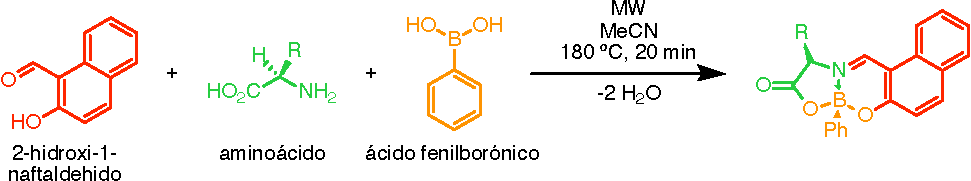
\includegraphics[width=0.85\linewidth]{./Figuras/BO-General.pdf}
        \caption[Síntesis de las BOSCHIBA por MW]{Método de síntesis para las \gls{BOSCHIBA} \textbf{1-4} por \gls{MW}.}
        \label{sch:reac-gral}
    \end{scheme}
    
    \subsubsection{Determinación de propiedades ópticas}
    \begin{itemize}[<+- | alert@+>]
        \item Se determinará el rendimiento cuántico de los compuestos \textbf{1-4}, así como su contraste de fluorescencia en medios de viscosidad variable.
    \end{itemize}
    
    \subsubsection{Determinación de citotoxicidad}
    \begin{itemize}
        \item Se determinará la citotoxicidad de los compuestos \textbf{1-4} en la línea celular de melanoma murino \emph{B16F10} (ATCC® CCL-6475™) derivado de ratón C57BL/6J.
    \end{itemize}
    
    \subsubsection{Modelado molecular}
    \begin{itemize}[<+- | alert@+>]
        \item Se realizarán cálculos \insilico{} por medio de \gls{DFT} y \gls{TDDFT} para estudiar las propiedades fotofísicas de los compuestos y comprobar los mecanismos involucrados en el efecto supresor de la luminiscencia en dichos compuestos así como estudios de topológicos sobre estos.
        \item En caso de no contar con datos cristalográficos en el momento del estudio \insilico{}, se hará una búsqueda conformacional con ayuda del programa \gls{CREST} \cite{prachtAutomatedExplorationLowenergy2020} para obtener los conformeros más estables de los compuestos.
        \item En caso de que se cuenten con datos cristalográficos, se utilizarán las coordenadas de la estructura cristalográfica para realizar la optimización geométrica en DFT.
        \item Se hará la optimización geométrica de los compuestos \textbf{1-4} empleando el funcional meta-GGA \scan{} \cite{gasevicOptimizationSCAN3cComposite2022} hasta llegar a un nivel de teoría de DFT/def2-TZVP, o superior en caso de que sea necesario.
        \item Se obtendrá el espectro de emisión de los compuestos \textbf{1-4} por medio de cálculos \gls{TDDFT} con el funcional ωB97X-V y con el fin de aproximarse al límite CBS, se requiere de aumentación con funciones difusas dobles, por lo que se usará el conjunto de funciones base def2-TZVPD o def2-QZVPPD si es necesario obtener estados de Rydberg.
    \end{itemize}
\end{frame}

\begin{frame}[allowframebreaks]{Referencias}
	\small
	\printbibliography{}
\end{frame}

\begin{frame}[allowframebreaks]{Glosario}
	\small
	% \printglossaries[nonumberlist]{}
	\printglossary[type=main,style=long,nonumberlist]
\end{frame}

\end{document}
